\documentclass[twoside]{book}

% Packages required by doxygen
\usepackage{fixltx2e}
\usepackage{calc}
\usepackage{doxygen}
\usepackage[export]{adjustbox} % also loads graphicx
\usepackage{graphicx}
\usepackage[utf8]{inputenc}
\usepackage{makeidx}
\usepackage{multicol}
\usepackage{multirow}
\PassOptionsToPackage{warn}{textcomp}
\usepackage{textcomp}
\usepackage[nointegrals]{wasysym}
\usepackage[table]{xcolor}

% NLS support packages
Portuguese
% Font selection
\usepackage[T1]{fontenc}
\usepackage[scaled=.90]{helvet}
\usepackage{courier}
\usepackage{amssymb}
\usepackage{sectsty}
\renewcommand{\familydefault}{\sfdefault}
\allsectionsfont{%
  \fontseries{bc}\selectfont%
  \color{darkgray}%
}
\renewcommand{\DoxyLabelFont}{%
  \fontseries{bc}\selectfont%
  \color{darkgray}%
}
\newcommand{\+}{\discretionary{\mbox{\scriptsize$\hookleftarrow$}}{}{}}

% Page & text layout
\usepackage{geometry}
\geometry{%
  a4paper,%
  top=2.5cm,%
  bottom=2.5cm,%
  left=2.5cm,%
  right=2.5cm%
}
\tolerance=750
\hfuzz=15pt
\hbadness=750
\setlength{\emergencystretch}{15pt}
\setlength{\parindent}{0cm}
\setlength{\parskip}{3ex plus 2ex minus 2ex}
\makeatletter
\renewcommand{\paragraph}{%
  \@startsection{paragraph}{4}{0ex}{-1.0ex}{1.0ex}{%
    \normalfont\normalsize\bfseries\SS@parafont%
  }%
}
\renewcommand{\subparagraph}{%
  \@startsection{subparagraph}{5}{0ex}{-1.0ex}{1.0ex}{%
    \normalfont\normalsize\bfseries\SS@subparafont%
  }%
}
\makeatother

% Headers & footers
\usepackage{fancyhdr}
\pagestyle{fancyplain}
\fancyhead[LE]{\fancyplain{}{\bfseries\thepage}}
\fancyhead[CE]{\fancyplain{}{}}
\fancyhead[RE]{\fancyplain{}{\bfseries\leftmark}}
\fancyhead[LO]{\fancyplain{}{\bfseries\rightmark}}
\fancyhead[CO]{\fancyplain{}{}}
\fancyhead[RO]{\fancyplain{}{\bfseries\thepage}}
\fancyfoot[LE]{\fancyplain{}{}}
\fancyfoot[CE]{\fancyplain{}{}}
\fancyfoot[RE]{\fancyplain{}{\bfseries\scriptsize Gerado por Doxygen }}
\fancyfoot[LO]{\fancyplain{}{\bfseries\scriptsize Gerado por Doxygen }}
\fancyfoot[CO]{\fancyplain{}{}}
\fancyfoot[RO]{\fancyplain{}{}}
\renewcommand{\footrulewidth}{0.4pt}
\renewcommand{\chaptermark}[1]{%
  \markboth{#1}{}%
}
\renewcommand{\sectionmark}[1]{%
  \markright{\thesection\ #1}%
}

% Indices & bibliography
\usepackage{natbib}
\usepackage[titles]{tocloft}
\setcounter{tocdepth}{3}
\setcounter{secnumdepth}{5}
\makeindex

% Hyperlinks (required, but should be loaded last)
\usepackage{ifpdf}
\ifpdf
  \usepackage[pdftex,pagebackref=true]{hyperref}
\else
  \usepackage[ps2pdf,pagebackref=true]{hyperref}
\fi
\hypersetup{%
  colorlinks=true,%
  linkcolor=blue,%
  citecolor=blue,%
  unicode%
}

% Custom commands
\newcommand{\clearemptydoublepage}{%
  \newpage{\pagestyle{empty}\cleardoublepage}%
}

\usepackage{caption}
\captionsetup{labelsep=space,justification=centering,font={bf},singlelinecheck=off,skip=4pt,position=top}

%===== C O N T E N T S =====

\begin{document}

% Titlepage & ToC
\hypersetup{pageanchor=false,
             bookmarksnumbered=true,
             pdfencoding=unicode
            }
\pagenumbering{roman}
\begin{titlepage}
\vspace*{7cm}
\begin{center}%
{\Large Hub Lembrol \\[1ex]\large 0.\+01 }\\
\vspace*{1cm}
{\large Gerado por Doxygen 1.8.11}\\
\end{center}
\end{titlepage}
\clearemptydoublepage
\tableofcontents
\clearemptydoublepage
\pagenumbering{arabic}
\hypersetup{pageanchor=true}

%--- Begin generated contents ---
\chapter{Página principal}
\label{index}\hypertarget{index}{}\begin{center} \section*{Engenharia de Software e Sistemas para ~\newline
 Engenharia da Computação -\/ E\+S\+S/\+EC Cin U\+F\+PE }\end{center} 

\begin{center} \end{center} 

~\newline
 ~\newline


\subsection*{~~~~ ~~~~Plano de Projeto -\/ lembrol }

\subsubsection*{Introdução }

Uma preocupação constante ao sair de uma residência é se algo foi esquecido, seja um guarda-\/chuva, até algo mais grave como um gás ligado. Existem momentos que lembramos logo ao sair, outros em que estamos longe demais para retornar e ficamos preocupados.

lembrol é um sistema de monitorame-\/nto residencial que avisa ao usuário algo que ele não lembrou, seja uma ação ou objeto, a fim de minimizar a quantidade de acidentes domésticos.

Baseado na IoT, esse sistema se comunica com sensores dos quais respondem com informações do ambiente, essas informações são comparadas com os dados registrados no momento da instalação, tudo que é fora do padrão é transformado em uma lista de ações que é mandada para o usuário em seu celular. Se o cliente sair de casa sem o dispositivo, um som gerado no lembrol alertará o usuário.

\subsubsection*{Organização do Projeto }



\tabulinesep=1mm
\begin{longtabu} spread 0pt [c]{*2{|X[-1]}|}
\hline
Área &Responsabilidades  \\\cline{1-2}
Gerente de Projeto &Definir, coordenar e integrar as atividades executadas para o desenvolvimento do projeto.  \\\cline{1-2}
Engenharia de Requisitos &Determinar, definir e gerenciar o estado e demais aspectos relacionados aos requisitos de software do sistema.  \\\cline{1-2}
Arquitetura de Sistemas &Desenhar e desenvolver a arquitetura dos sistemas.  \\\cline{1-2}
Desenvolvimento de Hardware &Projetar a arquitetura e desenvolver o hardware do projeto realizando os testes pertinentes.  \\\cline{1-2}
Desenvolvimento de Software &Projetar a arquitetura e desenvolver os componentes de software utilizados no projeto, realizando testes sob demanda.  \\\cline{1-2}
Gerência de Configuração e Mudanças &Controlar os artefatos produzidos pelos desenvolvedores e controlar os custos e esforços envolvidos na realização de uma mudança em um sistema.  \\\cline{1-2}
Engenharia de Testes &Criação de estratégias de teste com objetivo de validar os componentes do sistema durante e após seu desenvolvimento.  \\\cline{1-2}
User Interface Engineering &Desenvolver a parte de Interação com o usuário no sistema, para que fique da forma mais acessível o possível.  \\\cline{1-2}
\end{longtabu}


\subsubsection*{Análise de Riscos }

A análise a seguir leva em consideração os riscos identificados e sua categorização através dos valores atribuídos para as variáveis {\itshape severidade} e $\ast$probabilidade $\ast$de ocorrência. Esses atributos podem assumir valores em uma escala definida de 1 a 3, sendo o cálculo do risco dado pela seguinte multiplicação\+:

R\+I\+S\+CO = S\+E\+V\+E\+R\+I\+D\+A\+DE x P\+R\+O\+B\+A\+B\+I\+L\+I\+D\+A\+DE

Com base nas métricas definidas anteriormente e nos riscos potenciais evidenciados durante a etapa de levantamento foi possível consolidar a seguinte tabela\+:

\tabulinesep=1mm
\begin{longtabu} spread 0pt [c]{*5{|X[-1]}|}
\hline
Código &Descrição &Severidade &Probabilidade &Risco  \\\cline{1-5}
R1 &Problemas com a integração da central com os diferentes módulos do projeto &3 &2 &6  \\\cline{1-5}
R2 &Atrasos relacionados ao aprendizado das diferentes tecnologias envolvidas. &2 &3 &6  \\\cline{1-5}
R3 &Atrasos na entrega dos dispositivos de hardware solicitados / adquiridos. &3 &1 &3  \\\cline{1-5}
R4 &Mudança de requisitos de software / hardware envolvidos no projeto. &2 &2 &4  \\\cline{1-5}
R5 &Abandono de integrante devido a desistência de participação no projeto &2 &1 &2  \\\cline{1-5}
R6 &Integrante ficar doente &3 &2 &6  \\\cline{1-5}
\end{longtabu}


A seguir será apresentada uma breve descrição a respeito de possíveis ações associadas a cada um desses riscos. O objetivo é descrever as principais medidas para mitigá-\/los e como agir no caso da ocorrência de um incidente.

{\itshape R1 -\/ Problemas com a integração dos diferentes componentes de hardware e software.}


\begin{DoxyItemize}
\item Como mitigar o risco\+: A equipe deve procurar escolher tecnologias conhecidas para evitar erros causados pela falta de conhecimento nas plataformas de desenvolvimento. Além disso, é importante ficar atento a possíveis incompatibilidades que possam impactar e inviabilizar o desenvolvimento do projeto.
\item Ocorrência do incidente\+: Inicialmente pode-\/se alocar mais desenvolvedores para tentar resolver o problema de integração. Caso as dificuldades persistam, deve-\/se partir para tentar encontrar outras alternativas, como por exemplo, alterar os componentes de software ou de hardware e realizar ajustes.
\end{DoxyItemize}

{\itshape R2 -\/ Atrasos relacionados ao aprendizado das diferentes tecnologias envolvidas.}


\begin{DoxyItemize}
\item Como mitigar o risco\+: Escolher pessoas qualificadas para cada tarefa e que tenham engajamento dentro da sua área de atuação. Além disso, deve-\/se buscar ferramentas que proporcionem agilidade ao desenvolvimento garantindo que as atividades sejam cumpridas no tempo estimado.
\item Ocorrência do incidente\+: Deve-\/se alocar mais desenvolvedores para ajudar na tarefa e/ou auxiliar o desenvolvedor que está com dificuldades. Caso o problema persista, pode-\/se realocar o desenvolvedor com dificuldades para trabalhar em uma atividade diferente, que envolva uma tecnologia a qual ele está mais bem ambientado.
\end{DoxyItemize}

{\itshape R3 -\/ Atrasos na entrega dos dispositivos de hardware / software solicitados.}


\begin{DoxyItemize}
\item Como mitigar o risco\+: Realizar a decisão e pedido dos dispositivos com antecedência, minimizando assim eventuais riscos de atraso. Além disso, deve-\/se buscar alternativas na concepção inicial do projeto de modo a minimizar a dependência de um hardware específico, criando alternativas e maximizando o número de fornecedores.
\item Ocorrência do incidente\+: Buscar dentre as alternativas existentes um outro fornecedor, com disponibilidade de entrega imediata. Deve-\/se ainda adaptar, conforme necessário, os requisitos de hardware utilizados na concepção inicial do projeto.
\end{DoxyItemize}

{\itshape R4 -\/ Mudança de requisitos de software / hardware envolvidos no projeto.}


\begin{DoxyItemize}
\item Como mitigar o risco\+: Realizar uma pesquisa exaustiva durante o período inicial do projeto com foco na definição de requisitos sólidos, minimizando dessa forma a ocorrência de eventuais incompatibilidades durante a etapa de desenvolvimento.
\item Ocorrência do incidente\+: Certificar-\/se que a mudança é realmente necessária e definir corretamente o novo requisito, mapeando adequadamente o impacto nos demais requisitos do projeto e minimizando o risco de alterações futuras.
\end{DoxyItemize}

{\itshape R5 -\/ Abandono de integrante devido a desistência de participação no projeto.}


\begin{DoxyItemize}
\item Como mitigar o risco\+: Realizar um acompanhamento periódico das atividades realizadas, certificando-\/se que todos os membros da equipe tenham acesso ao material e o suporte necessário durante todo o desenvolvimento do projeto.
\item Ocorrência do incidente\+: Minimizar o impacto a partir da alocação de um outro desenvolvedor para área desfalcada. Negociar com o membro desistente a transferência do conhecimento e das responsabilidades envolvidas.
\end{DoxyItemize}

{\itshape R5 -\/ Integrante ficar doente}


\begin{DoxyItemize}
\item Como mitigar o risco\+: Evitar comidas estragadas, usar repelente, ser mais higiênico.
\item Ocorrência do incidente\+: Minimizar o impacto a partir da alocação de um outro desenvolvedor para área desfalcada. Pedir ao membro doente a transferência do conhecimento e das responsabilidades envolvidas.
\end{DoxyItemize}

\subsubsection*{Requisitos de recursos de hardware e software }

Foram mapeados os seguintes requisitos com relação aos recursos mínimos de hardware e software necessários para o desenvolvimento das atividades do projeto.


\begin{DoxyItemize}
\item Raspberry Pi\+: Será utilizada uma Raspberry Pi para atuar como coração do H\+UB..
\item Arduino Nano\+: Serão necessários dois Arduinos Nano para efetuar o processamento de dados necessário em cada módulo.
\item Resistores e Jumpers\+: Utilizados no desenvolvimento do circuito montado na protoboard. Necessários para efetuar a automação e o controle dos sensores que irão monitorar o ambiente.
\item Sensor de gás\+: Utilizado para detecção de vazamento de gás. Capta o nível de gás no ar, transformando em uma leitura analógica.
\item Piezzo elétrico \+: Reconhece quando há ou não há um peso acima do mesmo. Necessário para saber se o objeto importante está no lugar desejado ou não.
\item Swift\+: Linguagem open source utilizada para desenvolvimento em plataformas da Apple de fácil legibilidade e redigibilidade. Necessária para programação do aplicativo i\+OS.
\item Firebase \+: Serviço de nuvem para banco de dados em tempo real, com A\+PI para diversas linguagens, permite que mudanças no banco de dados possam ser acompanhadas de forma simples
\item Python \+: Linguagem open source conhecida por ser extremamente simples e fácil de entender. Necessária para programação da Raspberry Pi.
\item Baterias Lipo \+: Baterias para funcionamento do sistema em modo remoto. Necessárias para garantir autonomia do sistema.
\item E\+S\+P8266 \+: Módulo Wi\+Fi para conexão de internet para Arduino. Necessário para passagem de dados entre o H\+UB e os módulos.
\end{DoxyItemize}

\subsubsection*{Estrutura Analítica }

Com base nas reuniões efetuadas para discussão sobre o processo de divisão de atividades foram identificadas as seguintes estruturas analíticas para o projeto.

{\itshape T1 -\/ Fazer requisitos}

Detalhar os requisitos de serviços funcionais e não funcionais, de forma, detalhada e registrar todos os requisitos.

{\itshape T2 -\/ Montar os casos de uso}

Descrever os casos de uso para serem consultados durante todo o desenvolvimento.

{\itshape T3 -\/ Montar a arquitetura do H\+UB}

Arquitetar o H\+UB, arquitetura deve conter todo o sistema do H\+UB que será o centro do serviço e deve se conectar com todos os componentes e usuários do sistema. A sua arquitetura deve ser bem montada para sua comunicação.

{\itshape T4 -\/ Modelar comunicação do H\+UB}

Modelar a comunicação do H\+UB com módulos e aplicativos, para uma comunicação efetiva e sem atrasos, feita com diversos testes no sistema

{\itshape T5 -\/ Modelar banco de dados do H\+UB}

Modelar o banco de dados onde os estados dos sensores vão ser armazenados para em seguida serem enviadas para o aplicativo e serem visualizados pelo usuário.

{\itshape T6 -\/ Desenvolver aplicativo}

Desenvolver aplicativo de gerenciamento do sistema pelo usuário, o aplicativo deverá informar ao usuário o estado dos sensores, se comunicar com o H\+UB e seu banco de dados além de informar ao H\+UB sua localização para análise de esquecimento do dispositivo.

{\itshape T7 -\/ Montar hardware do módulo de objetos importantes}

Desenvolver módulo de localização para hardware que será colocado em objetos que possuem grande importância e não poderão ser esquecidos pelo usuário.

O módulo deve estar anexado ao objeto e o usuário deve ser alertado caso saia de sua residência e esqueça o objeto, no caso do celular a sua posição será feita pelo aplicativo.

{\itshape T8 -\/ Desenvolver o software do módulo de objetos importantes}

Desenvolver software de comunicação do módulo com o H\+UB, leitura de dados e envio para o H\+UB, que armazenará seu estado em seu banco de dados.

{\itshape T9 -\/ Integração do módulo de objetos importantes com o H\+UB}

Integração do módulo e com o H\+UB deve ser feita de forma com que o módulo possa ser facilmente removido e adicionado. Sua comunicação deve ser feita para uma interação rápida e deve ser amplamente testada.

{\itshape T10 -\/ Montar o módulo de gás}

Desenvolver o módulo de gás e sua comunicação com o H\+UB, suas funcionalidades e suas conexões

{\itshape T11 -\/ Desenvolver o software do módulo de gás}

{\itshape Desenvolver software de leitura, análise e envio de dados do módulo.}

{\itshape T12 -\/ Integrar o módulo de gás com o H\+UB}

Conectar o módulo com o H\+UB, testar funcionalidades e comunicação entre H\+UB e módulos.

\subsubsection*{Cronograma do Projeto }

Com base nas estruturas analíticas do projeto foi estabelecido o seguinte cronograma.

\tabulinesep=1mm
\begin{longtabu} spread 0pt [c]{*4{|X[-1]}|}
\hline
Atividade &Entrega &Responsáveis &Dependências  \\\cline{1-4}
T1 &12/10/2016 &hcf2 &-\/  \\\cline{1-4}
T2 &12/10/2016 &hcf2 &T1  \\\cline{1-4}
T3 &26/10/2016 &mpmr,jnolj &T2  \\\cline{1-4}
T4 &26/10/2016 &mpmr,jnolj &T3  \\\cline{1-4}
T5 &26/10/2016 &mpmr,jnolj &T3  \\\cline{1-4}
T6 &14/11/2016 &jnolj &T5  \\\cline{1-4}
T7 &21/11/2016 &dapd,mapa &T1  \\\cline{1-4}
T8 &21/11/2016 &dapd,mapa,jnolj,mpmr &T7  \\\cline{1-4}
T9 &21/11/2016 &dapd,mapa,jnolj,mpmr &T8  \\\cline{1-4}
T10 &05/12/2016 &dapd,mapa &T1  \\\cline{1-4}
T11 &05/12/2016 &dapd,mapa,jnolj,mpmr &T10  \\\cline{1-4}
T12 &05/12/2016 &dapd,mapa,jnolj,mpmr &T11  \\\cline{1-4}
\end{longtabu}


\subsubsection*{Mecanismos de monitoramento e elaboração de relatórios }

Ao longo do processo de desenvolvimento serão disponibilizados relatórios gerenciais para refletir o nível atual de progresso e andamento das atividades através de métricas bem definidas. Esses relatórios serão consolidados em cada milestone e servirão de instrumento fundamental para o acompanhamento do projeto pelas partes interessadas.

Com base no cronograma apresentado serão definidas atividades elementares para representar as etapas de desenvolvimento necessárias para alcançar os milestones definidos. Cada atividade terá uma prioridade para execução, uma estimativa de esforço, além de um responsável pelo desenvolvimento.

O registro global dessas atividades com relação ao progresso e a rastreabilidade serão efetuados através de ferramentas auxiliares, notadamente o Trello \mbox{[}1\mbox{]} e o Git\+Hub \mbox{[}2\mbox{]}. A primeira proporciona uma visão gerencial dando indicativos claros a respeito do progresso efetuado, enquanto a segunda permite um acompanhamento operacional, fornecendo indicadores essenciais que orientam o processo de gestão de mudanças.

Referências

\mbox{[}1\mbox{]} \href{http://www.trello.com}{\tt http\+://www.\+trello.\+com}

\mbox{[}2\mbox{]} \href{https://github.com/}{\tt https\+://github.\+com/} 
\chapter{Índice da hierarquia}
\section{Hierarquia de classes}
Esta lista de heranças está organizada, dentro do possível, por ordem alfabética\+:\begin{DoxyCompactList}
\item Device\begin{DoxyCompactList}
\item \contentsline{section}{adaptador\+Bluetooth.\+Adaptador\+Bluetooth}{\pageref{classadaptador_bluetooth_1_1_adaptador_bluetooth}}{}
\end{DoxyCompactList}
\item object\begin{DoxyCompactList}
\item \contentsline{section}{controlador\+Bluetooh.\+Controlador\+Bluetooh}{\pageref{classcontrolador_bluetooh_1_1_controlador_bluetooh}}{}
\item \contentsline{section}{device.\+Device}{\pageref{classdevice_1_1_device}}{}
\item \contentsline{section}{hub.\+Hub}{\pageref{classhub_1_1_hub}}{}
\item \contentsline{section}{hub\+Para\+Firebase.\+Hub\+Para\+Firebase}{\pageref{classhub_para_firebase_1_1_hub_para_firebase}}{}
\item \contentsline{section}{hub\+Para\+Modulo.\+Hub\+Para\+Modulo}{\pageref{classhub_para_modulo_1_1_hub_para_modulo}}{}
\item \contentsline{section}{led\+Manager.\+Led\+Manager}{\pageref{classled_manager_1_1_led_manager}}{}
\item \contentsline{section}{led\+Manager.\+R\+GB}{\pageref{classled_manager_1_1_r_g_b}}{}
\end{DoxyCompactList}
\end{DoxyCompactList}

\chapter{Índice dos componentes}
\section{Lista de componentes}
Lista de classes, estruturas, uniões e interfaces com uma breve descrição\+:\begin{DoxyCompactList}
\item\contentsline{section}{\hyperlink{classadaptador_bluetooth_1_1_adaptador_bluetooth}{adaptador\+Bluetooth.\+Adaptador\+Bluetooth} \\*Class for adaptador bluetooth }{\pageref{classadaptador_bluetooth_1_1_adaptador_bluetooth}}{}
\item\contentsline{section}{\hyperlink{classcontrolador_bluetooh_1_1_controlador_bluetooh}{controlador\+Bluetooh.\+Controlador\+Bluetooh} }{\pageref{classcontrolador_bluetooh_1_1_controlador_bluetooh}}{}
\item\contentsline{section}{\hyperlink{classdevice_1_1_device}{device.\+Device} \\*Class for device }{\pageref{classdevice_1_1_device}}{}
\item\contentsline{section}{\hyperlink{classhub_1_1_hub}{hub.\+Hub} \\*Classe para o H\+UB }{\pageref{classhub_1_1_hub}}{}
\item\contentsline{section}{\hyperlink{classhub_para_firebase_1_1_hub_para_firebase}{hub\+Para\+Firebase.\+Hub\+Para\+Firebase} \\*Class for hub para firebase }{\pageref{classhub_para_firebase_1_1_hub_para_firebase}}{}
\item\contentsline{section}{\hyperlink{classhub_para_modulo_1_1_hub_para_modulo}{hub\+Para\+Modulo.\+Hub\+Para\+Modulo} \\*Class for hub para modulo }{\pageref{classhub_para_modulo_1_1_hub_para_modulo}}{}
\item\contentsline{section}{\hyperlink{classled_manager_1_1_led_manager}{led\+Manager.\+Led\+Manager} \\*Classe para o \hyperlink{classled_manager_1_1_led_manager}{Led\+Manager} }{\pageref{classled_manager_1_1_led_manager}}{}
\item\contentsline{section}{\hyperlink{classled_manager_1_1_r_g_b}{led\+Manager.\+R\+GB} \\*Classe para rgb }{\pageref{classled_manager_1_1_r_g_b}}{}
\end{DoxyCompactList}

\chapter{Documentação da classe}
\hypertarget{classadaptador_bluetooth_1_1_adaptador_bluetooth}{}\section{Referência à classe adaptador\+Bluetooth.\+Adaptador\+Bluetooth}
\label{classadaptador_bluetooth_1_1_adaptador_bluetooth}\index{adaptador\+Bluetooth.\+Adaptador\+Bluetooth@{adaptador\+Bluetooth.\+Adaptador\+Bluetooth}}


Class for adaptador bluetooth.  


Diagrama de heranças da classe adaptador\+Bluetooth.\+Adaptador\+Bluetooth\begin{figure}[H]
\begin{center}
\leavevmode
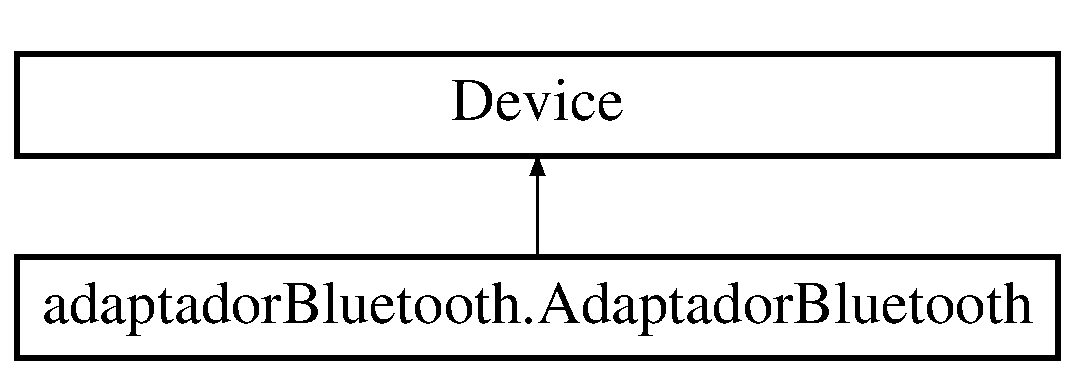
\includegraphics[height=2.000000cm]{classadaptador_bluetooth_1_1_adaptador_bluetooth}
\end{center}
\end{figure}
\subsection*{Membros públicos}
\begin{DoxyCompactItemize}
\item 
def \hyperlink{classadaptador_bluetooth_1_1_adaptador_bluetooth_a11e812b23e047752d56486e4b327077d}{\+\_\+\+\_\+init\+\_\+\+\_\+} (self, arg)
\begin{DoxyCompactList}\small\item\em Constructs the object. \end{DoxyCompactList}\item 
def \hyperlink{classadaptador_bluetooth_1_1_adaptador_bluetooth_a9c32b04776ece3fdc29dd9b88c006d73}{parear} ()
\begin{DoxyCompactList}\small\item\em \{ function\+\_\+description \} \end{DoxyCompactList}\item 
def \hyperlink{classadaptador_bluetooth_1_1_adaptador_bluetooth_aeb85cf48ef2abf3bdcd0135aa6765078}{tornar\+Visivel} ()
\begin{DoxyCompactList}\small\item\em \{ function\+\_\+description \} \end{DoxyCompactList}\end{DoxyCompactItemize}
\subsection*{Atributos Públicos}
\begin{DoxyCompactItemize}
\item 
{\bfseries arg}\hypertarget{classadaptador_bluetooth_1_1_adaptador_bluetooth_aa9722fd9312eed3e2a3143d3a594aa9f}{}\label{classadaptador_bluetooth_1_1_adaptador_bluetooth_aa9722fd9312eed3e2a3143d3a594aa9f}

\end{DoxyCompactItemize}
\subsection*{Atributos Públicos Estáticos}
\begin{DoxyCompactItemize}
\item 
int {\bfseries pin} = 0\hypertarget{classadaptador_bluetooth_1_1_adaptador_bluetooth_a8bd31f3c5c66b219d16cd6f945d0265f}{}\label{classadaptador_bluetooth_1_1_adaptador_bluetooth_a8bd31f3c5c66b219d16cd6f945d0265f}

\end{DoxyCompactItemize}


\subsection{Descrição detalhada}
Class for adaptador bluetooth. 


\begin{DoxyParams}{Parâmetros}
{\em pin} & The pin \\
\hline
{\em \+\_\+id} & The id \\
\hline
\end{DoxyParams}


\subsection{Documentação dos Construtores \& Destrutor}
\index{adaptador\+Bluetooth\+::\+Adaptador\+Bluetooth@{adaptador\+Bluetooth\+::\+Adaptador\+Bluetooth}!\+\_\+\+\_\+init\+\_\+\+\_\+@{\+\_\+\+\_\+init\+\_\+\+\_\+}}
\index{\+\_\+\+\_\+init\+\_\+\+\_\+@{\+\_\+\+\_\+init\+\_\+\+\_\+}!adaptador\+Bluetooth\+::\+Adaptador\+Bluetooth@{adaptador\+Bluetooth\+::\+Adaptador\+Bluetooth}}
\subsubsection[{\texorpdfstring{\+\_\+\+\_\+init\+\_\+\+\_\+(self, arg)}{__init__(self, arg)}}]{\setlength{\rightskip}{0pt plus 5cm}def adaptador\+Bluetooth.\+Adaptador\+Bluetooth.\+\_\+\+\_\+init\+\_\+\+\_\+ (
\begin{DoxyParamCaption}
\item[{}]{self, }
\item[{}]{arg}
\end{DoxyParamCaption}
)}\hypertarget{classadaptador_bluetooth_1_1_adaptador_bluetooth_a11e812b23e047752d56486e4b327077d}{}\label{classadaptador_bluetooth_1_1_adaptador_bluetooth_a11e812b23e047752d56486e4b327077d}


Constructs the object. 


\begin{DoxyParams}{Parâmetros}
{\em self} & The object \\
\hline
{\em arg} & The argument \\
\hline
\end{DoxyParams}


\subsection{Documentação dos métodos}
\index{adaptador\+Bluetooth\+::\+Adaptador\+Bluetooth@{adaptador\+Bluetooth\+::\+Adaptador\+Bluetooth}!parear@{parear}}
\index{parear@{parear}!adaptador\+Bluetooth\+::\+Adaptador\+Bluetooth@{adaptador\+Bluetooth\+::\+Adaptador\+Bluetooth}}
\subsubsection[{\texorpdfstring{parear()}{parear()}}]{\setlength{\rightskip}{0pt plus 5cm}def adaptador\+Bluetooth.\+Adaptador\+Bluetooth.\+parear (
\begin{DoxyParamCaption}
{}
\end{DoxyParamCaption}
)}\hypertarget{classadaptador_bluetooth_1_1_adaptador_bluetooth_a9c32b04776ece3fdc29dd9b88c006d73}{}\label{classadaptador_bluetooth_1_1_adaptador_bluetooth_a9c32b04776ece3fdc29dd9b88c006d73}


\{ function\+\_\+description \} 

\begin{DoxyReturn}{Retorna}
\{ description\+\_\+of\+\_\+the\+\_\+return\+\_\+value \} 
\end{DoxyReturn}
\index{adaptador\+Bluetooth\+::\+Adaptador\+Bluetooth@{adaptador\+Bluetooth\+::\+Adaptador\+Bluetooth}!tornar\+Visivel@{tornar\+Visivel}}
\index{tornar\+Visivel@{tornar\+Visivel}!adaptador\+Bluetooth\+::\+Adaptador\+Bluetooth@{adaptador\+Bluetooth\+::\+Adaptador\+Bluetooth}}
\subsubsection[{\texorpdfstring{tornar\+Visivel()}{tornarVisivel()}}]{\setlength{\rightskip}{0pt plus 5cm}def adaptador\+Bluetooth.\+Adaptador\+Bluetooth.\+tornar\+Visivel (
\begin{DoxyParamCaption}
{}
\end{DoxyParamCaption}
)}\hypertarget{classadaptador_bluetooth_1_1_adaptador_bluetooth_aeb85cf48ef2abf3bdcd0135aa6765078}{}\label{classadaptador_bluetooth_1_1_adaptador_bluetooth_aeb85cf48ef2abf3bdcd0135aa6765078}


\{ function\+\_\+description \} 

\begin{DoxyReturn}{Retorna}
\{ description\+\_\+of\+\_\+the\+\_\+return\+\_\+value \} 
\end{DoxyReturn}


A documentação para esta classe foi gerada a partir do seguinte ficheiro\+:\begin{DoxyCompactItemize}
\item 
adaptador\+Bluetooth.\+py\end{DoxyCompactItemize}

\hypertarget{classcontrolador_bluetooh_1_1_controlador_bluetooh}{}\section{Referência à classe controlador\+Bluetooh.\+Controlador\+Bluetooh}
\label{classcontrolador_bluetooh_1_1_controlador_bluetooh}\index{controlador\+Bluetooh.\+Controlador\+Bluetooh@{controlador\+Bluetooh.\+Controlador\+Bluetooh}}
Diagrama de heranças da classe controlador\+Bluetooh.\+Controlador\+Bluetooh\begin{figure}[H]
\begin{center}
\leavevmode
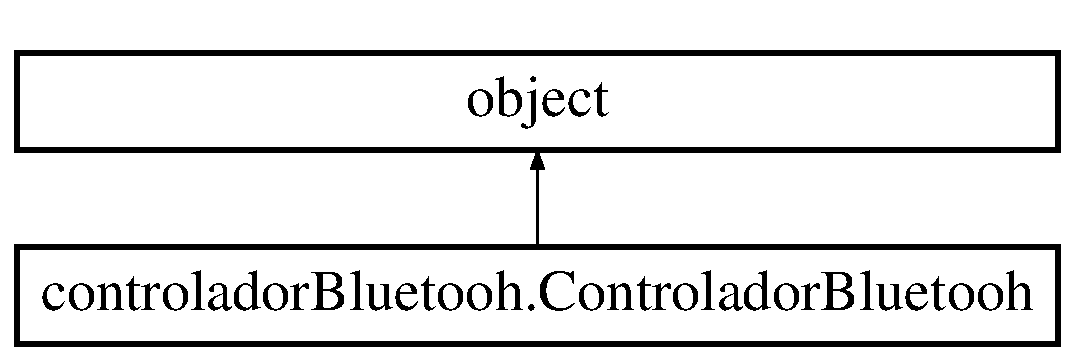
\includegraphics[height=2.000000cm]{classcontrolador_bluetooh_1_1_controlador_bluetooh}
\end{center}
\end{figure}
\subsection*{Membros públicos}
\begin{DoxyCompactItemize}
\item 
def {\bfseries \+\_\+\+\_\+init\+\_\+\+\_\+} (self, arg)\hypertarget{classcontrolador_bluetooh_1_1_controlador_bluetooh_a6b01f46d49cd95528274c008261fcf8d}{}\label{classcontrolador_bluetooh_1_1_controlador_bluetooh_a6b01f46d49cd95528274c008261fcf8d}

\end{DoxyCompactItemize}
\subsection*{Atributos Públicos}
\begin{DoxyCompactItemize}
\item 
{\bfseries arg}\hypertarget{classcontrolador_bluetooh_1_1_controlador_bluetooh_ac15bab8b920b372149393c33bbb6a00d}{}\label{classcontrolador_bluetooh_1_1_controlador_bluetooh_ac15bab8b920b372149393c33bbb6a00d}

\end{DoxyCompactItemize}


A documentação para esta classe foi gerada a partir do seguinte ficheiro\+:\begin{DoxyCompactItemize}
\item 
controlador\+Bluetooh.\+py\end{DoxyCompactItemize}

\hypertarget{classdevice_1_1_device}{}\section{Referência à classe device.\+Device}
\label{classdevice_1_1_device}\index{device.\+Device@{device.\+Device}}


Classe para \hyperlink{classdevice_1_1_device}{Device}.  


Diagrama de heranças da classe device.\+Device\begin{figure}[H]
\begin{center}
\leavevmode
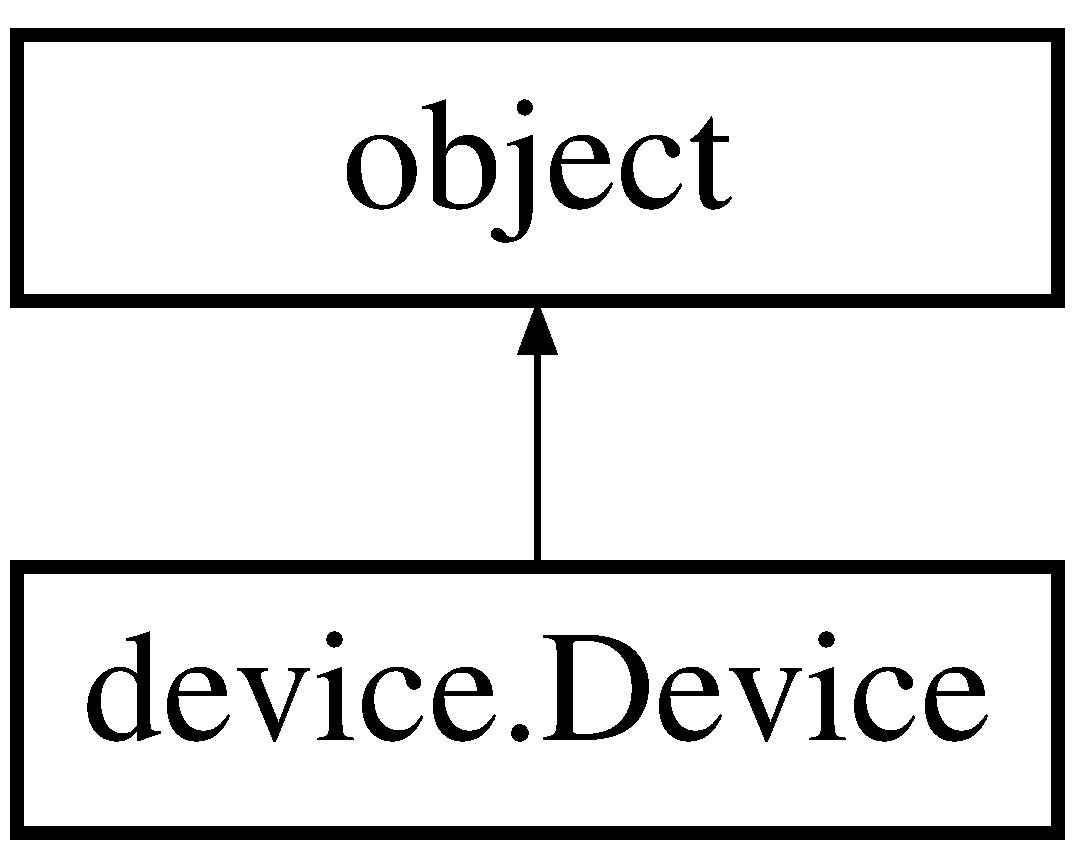
\includegraphics[height=2.000000cm]{classdevice_1_1_device}
\end{center}
\end{figure}
\subsection*{Membros públicos}
\begin{DoxyCompactItemize}
\item 
def \hyperlink{classdevice_1_1_device_a6ed267a3bacc28a17a6dc910167b1ca2}{\+\_\+\+\_\+init\+\_\+\+\_\+} (self, arg)
\begin{DoxyCompactList}\small\item\em Constrói o objeto. \end{DoxyCompactList}\end{DoxyCompactItemize}
\subsection*{Atributos Públicos}
\begin{DoxyCompactItemize}
\item 
{\bfseries arg}\hypertarget{classdevice_1_1_device_a0dca5f5fca68b9e9c63e238fbc21c84d}{}\label{classdevice_1_1_device_a0dca5f5fca68b9e9c63e238fbc21c84d}

\end{DoxyCompactItemize}


\subsection{Descrição detalhada}
Classe para \hyperlink{classdevice_1_1_device}{Device}. 

\subsection{Documentação dos Construtores \& Destrutor}
\index{device\+::\+Device@{device\+::\+Device}!\+\_\+\+\_\+init\+\_\+\+\_\+@{\+\_\+\+\_\+init\+\_\+\+\_\+}}
\index{\+\_\+\+\_\+init\+\_\+\+\_\+@{\+\_\+\+\_\+init\+\_\+\+\_\+}!device\+::\+Device@{device\+::\+Device}}
\subsubsection[{\texorpdfstring{\+\_\+\+\_\+init\+\_\+\+\_\+(self, arg)}{__init__(self, arg)}}]{\setlength{\rightskip}{0pt plus 5cm}def device.\+Device.\+\_\+\+\_\+init\+\_\+\+\_\+ (
\begin{DoxyParamCaption}
\item[{}]{self, }
\item[{}]{arg}
\end{DoxyParamCaption}
)}\hypertarget{classdevice_1_1_device_a6ed267a3bacc28a17a6dc910167b1ca2}{}\label{classdevice_1_1_device_a6ed267a3bacc28a17a6dc910167b1ca2}


Constrói o objeto. 


\begin{DoxyParams}{Parâmetros}
{\em self} & O objeto \\
\hline
{\em arg} & O argumento \\
\hline
\end{DoxyParams}


A documentação para esta classe foi gerada a partir do seguinte ficheiro\+:\begin{DoxyCompactItemize}
\item 
device.\+py\end{DoxyCompactItemize}

\hypertarget{classhub_1_1_hub}{}\section{Referência à classe hub.\+Hub}
\label{classhub_1_1_hub}\index{hub.\+Hub@{hub.\+Hub}}


Classe para o H\+UB.  


Diagrama de heranças da classe hub.\+Hub\begin{figure}[H]
\begin{center}
\leavevmode
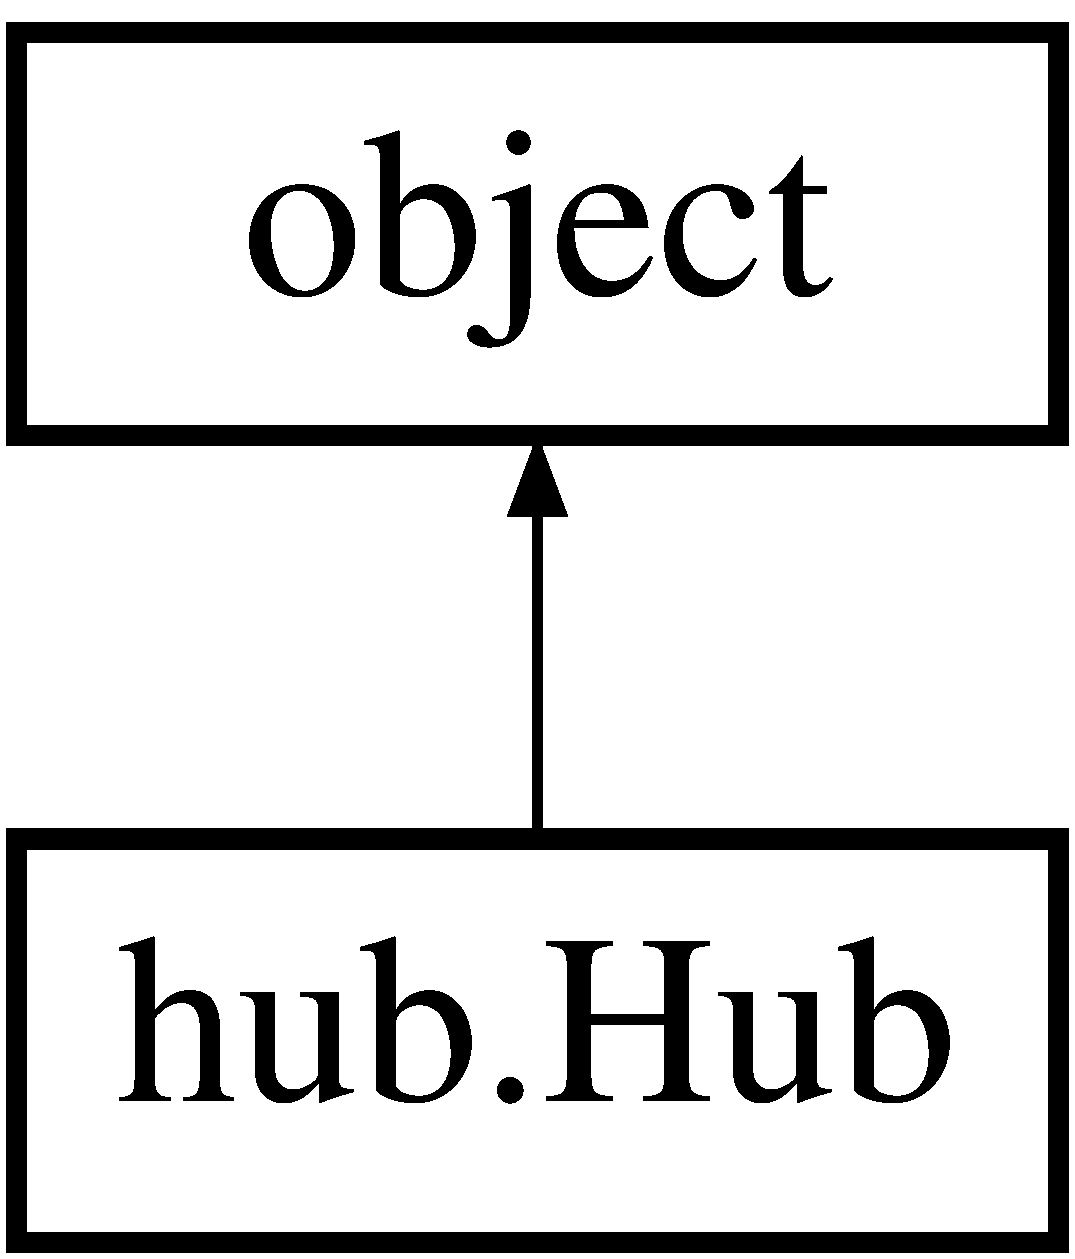
\includegraphics[height=2.000000cm]{classhub_1_1_hub}
\end{center}
\end{figure}
\subsection*{Membros públicos}
\begin{DoxyCompactItemize}
\item 
def \hyperlink{classhub_1_1_hub_a6927b78580ea47e1525a945e7d1da004}{\+\_\+\+\_\+init\+\_\+\+\_\+} (self, status)
\begin{DoxyCompactList}\small\item\em Método de inicialização para o H\+UB. \end{DoxyCompactList}\item 
def \hyperlink{classhub_1_1_hub_a27a1a63e552a3cf6a6229e655ef4e368}{loop\+Principal} (self)
\begin{DoxyCompactList}\small\item\em Esse é o loop principal do H\+UB, onde será implementada sua máquina de estados. \end{DoxyCompactList}\item 
def \hyperlink{classhub_1_1_hub_a32160e972d5ac2c695a3e86816113b95}{configurar\+Primeira\+Vez} (self)
\begin{DoxyCompactList}\small\item\em Método configura o H\+UB no primeiro acesso. \end{DoxyCompactList}\item 
def \hyperlink{classhub_1_1_hub_a9b81ca32890f6df8dece0e1ae497ee20}{tocar\+Buzzer} (self)
\begin{DoxyCompactList}\small\item\em Método aciona o Buzzer. \end{DoxyCompactList}\item 
def \hyperlink{classhub_1_1_hub_ac549b975878cf88b96dfbc57c319193e}{acionar\+Led} (self)
\begin{DoxyCompactList}\small\item\em Método aciona o Led. \end{DoxyCompactList}\end{DoxyCompactItemize}
\subsection*{Atributos Públicos}
\begin{DoxyCompactItemize}
\item 
{\bfseries status}\hypertarget{classhub_1_1_hub_aca0fde3216b7d279e6619aed32bfa418}{}\label{classhub_1_1_hub_aca0fde3216b7d279e6619aed32bfa418}

\end{DoxyCompactItemize}
\subsection*{Atributos Públicos Estáticos}
\begin{DoxyCompactItemize}
\item 
string {\bfseries status} = \char`\"{}\char`\"{}\hypertarget{classhub_1_1_hub_a5b81b3d458d8bea39e1a6aa5122ae5f0}{}\label{classhub_1_1_hub_a5b81b3d458d8bea39e1a6aa5122ae5f0}

\item 
string {\bfseries U\+ID} = \char`\"{}\char`\"{}\hypertarget{classhub_1_1_hub_ab0675c400cb26d7ecf6c7e8216b38f88}{}\label{classhub_1_1_hub_ab0675c400cb26d7ecf6c7e8216b38f88}

\item 
{\bfseries led\+Manager} = None\hypertarget{classhub_1_1_hub_a1072169bef5f5cfc46957270c95ac0e3}{}\label{classhub_1_1_hub_a1072169bef5f5cfc46957270c95ac0e3}

\item 
{\bfseries hub\+Para\+Modulo} = None\hypertarget{classhub_1_1_hub_ad76ddaf14bf717d58801e482ec8170b5}{}\label{classhub_1_1_hub_ad76ddaf14bf717d58801e482ec8170b5}

\item 
{\bfseries hub\+Para\+Firebase} = None\hypertarget{classhub_1_1_hub_adeb7bfdecbaeb53c2b288e7e1fd9e7fd}{}\label{classhub_1_1_hub_adeb7bfdecbaeb53c2b288e7e1fd9e7fd}

\item 
{\bfseries adaptador\+Bluetooth} = None\hypertarget{classhub_1_1_hub_a1b5657982fcd346c9733253e842b0e82}{}\label{classhub_1_1_hub_a1b5657982fcd346c9733253e842b0e82}

\end{DoxyCompactItemize}


\subsection{Descrição detalhada}
Classe para o H\+UB. 

Nesta classe, espera-\/se que todos os métodos principais do H\+UB sejam devidamente escritos. O comportamento do H\+UB por enquanto se limita a um método que fica rodando em loop infinito, e de acordo com os estímulos recebidos das threads de {\itshape escutar}, executa ações, ou seja, é uma máquina de estados. É importante que os métodos de escutar das instâncias {\ttfamily hub\+Para\+Módulo} e {\ttfamily hub\+Para\+Firebase} rodem em paralelo como threads, e que haja um comportamento de produtor-\/consumidor quanto às informações obtidas e enviadas.

A convenção será\+: nome minúsculo para instâncias, variáveis e métodos, e nome maiúsculo para classes.

\begin{DoxyWarning}{Aviso}
Colocar verificações e erros caso algo aconteça, mas nunca paralizar ou fechar o programa. É importante que os erros sejam tratados.
\end{DoxyWarning}

\begin{DoxyParams}{Parâmetros}
{\em status} & O status do H\+UB. Uma string pré-\/definida. \\
\hline
{\em U\+ID} & O ID do usuário que cadastrou o H\+UB. Uma String. \\
\hline
{\em led\+Manager} & Instância da classe Led\+Manager. \\
\hline
{\em hub\+Para\+Modulo} & Instância da classe Hub\+Para\+Modulo. \\
\hline
{\em hub\+Para\+Firebase} & Instância da classe Hub\+Para\+Firebase. \\
\hline
{\em adaptador\+Bluetooth} & Instância da classe Adaptador\+Bluetooth. \\
\hline
\end{DoxyParams}


\subsection{Documentação dos Construtores \& Destrutor}
\index{hub\+::\+Hub@{hub\+::\+Hub}!\+\_\+\+\_\+init\+\_\+\+\_\+@{\+\_\+\+\_\+init\+\_\+\+\_\+}}
\index{\+\_\+\+\_\+init\+\_\+\+\_\+@{\+\_\+\+\_\+init\+\_\+\+\_\+}!hub\+::\+Hub@{hub\+::\+Hub}}
\subsubsection[{\texorpdfstring{\+\_\+\+\_\+init\+\_\+\+\_\+(self, status)}{__init__(self, status)}}]{\setlength{\rightskip}{0pt plus 5cm}def hub.\+Hub.\+\_\+\+\_\+init\+\_\+\+\_\+ (
\begin{DoxyParamCaption}
\item[{}]{self, }
\item[{}]{status}
\end{DoxyParamCaption}
)}\hypertarget{classhub_1_1_hub_a6927b78580ea47e1525a945e7d1da004}{}\label{classhub_1_1_hub_a6927b78580ea47e1525a945e7d1da004}


Método de inicialização para o H\+UB. 

O método de inicialização para o H\+UB recebe como entrada o valor inicial do status do H\+UB e retorna um booleano, que informa se a operação foi concluída com sucesso. Espera-\/se que após chamar essa função, todos os parâmetros do H\+UB estejam devidamente inicializados. Isso inclui parâmetros adicionados posteriormente por necessidade, ou seja, parâmetros auxiliares.

Para adicionar parâmetros auxiliares, adicione o mesmo em\+:


\begin{DoxyCode}
1 \textcolor{keyword}{def }\_\_init\_\_(self, status):
\end{DoxyCode}
 \begin{DoxyVerb}        Por exemplo, para adicionar o parâmetro aux (cujo nome não é
        recomendável de ser usado), deve-se fazer o seguinte:
\end{DoxyVerb}



\begin{DoxyCode}
1 \textcolor{keyword}{def} \_\_init\_\_(self, status, aux):
2  super(Hub, self).\_\_init\_\_()
3  self.status = status
4  self.aux = xpto
\end{DoxyCode}
 \begin{DoxyVerb}        Onde xpto é o valor inicial desejado.
\end{DoxyVerb}


\begin{DoxyWarning}{Aviso}
Inicializar instâncias de classes depois.
\end{DoxyWarning}

\begin{DoxyParams}{Parâmetros}
{\em self} & O objeto \\
\hline
{\em status} & O status do H\+UB. Uma string pré-\/definida. \\
\hline
\end{DoxyParams}


\subsection{Documentação dos métodos}
\index{hub\+::\+Hub@{hub\+::\+Hub}!acionar\+Led@{acionar\+Led}}
\index{acionar\+Led@{acionar\+Led}!hub\+::\+Hub@{hub\+::\+Hub}}
\subsubsection[{\texorpdfstring{acionar\+Led(self)}{acionarLed(self)}}]{\setlength{\rightskip}{0pt plus 5cm}def hub.\+Hub.\+acionar\+Led (
\begin{DoxyParamCaption}
\item[{}]{self}
\end{DoxyParamCaption}
)}\hypertarget{classhub_1_1_hub_ac549b975878cf88b96dfbc57c319193e}{}\label{classhub_1_1_hub_ac549b975878cf88b96dfbc57c319193e}


Método aciona o Led. 

Este método utiliza a instância {\ttfamily led\+Manager} que é atributo desta classe, e deve se comportar, utilizando o atributo {\ttfamily status} e chamando os métodos de ligar\+Led, desligar\+Led e procurar\+Significado da classe led\+Manager. Em resumo, ao chamar essa classe, é esperado que ela atualize o comportamento do led de acordo com o status atual.

\begin{DoxyReturn}{Retorna}
O valor de retorno sempre será {\ttfamily N\+U\+LL}. 
\end{DoxyReturn}
\index{hub\+::\+Hub@{hub\+::\+Hub}!configurar\+Primeira\+Vez@{configurar\+Primeira\+Vez}}
\index{configurar\+Primeira\+Vez@{configurar\+Primeira\+Vez}!hub\+::\+Hub@{hub\+::\+Hub}}
\subsubsection[{\texorpdfstring{configurar\+Primeira\+Vez(self)}{configurarPrimeiraVez(self)}}]{\setlength{\rightskip}{0pt plus 5cm}def hub.\+Hub.\+configurar\+Primeira\+Vez (
\begin{DoxyParamCaption}
\item[{}]{self}
\end{DoxyParamCaption}
)}\hypertarget{classhub_1_1_hub_a32160e972d5ac2c695a3e86816113b95}{}\label{classhub_1_1_hub_a32160e972d5ac2c695a3e86816113b95}


Método configura o H\+UB no primeiro acesso. 

No primeiro acesso ao H\+UB, o mesmo não estará cadastrado no servidor e, portanto, não estará anexado ao usuário. Espera-\/se que esse método realize uma coneção com o firebase, sem utilizar o respectivo objeto de coneção ao firebase. Ou seja, uma conexão simples ao firebase é realizada aqui. Espera-\/se receber através dessa conexão o U\+ID do usuário que adicionou este H\+UB.

\begin{DoxyReturn}{Retorna}
U\+ID do usuário que adicionou este H\+UB. 
\end{DoxyReturn}
\begin{DoxyWarning}{Aviso}
Modificar diagrama de blocos para que demonstre o que é retornado aqui. 
\end{DoxyWarning}
\index{hub\+::\+Hub@{hub\+::\+Hub}!loop\+Principal@{loop\+Principal}}
\index{loop\+Principal@{loop\+Principal}!hub\+::\+Hub@{hub\+::\+Hub}}
\subsubsection[{\texorpdfstring{loop\+Principal(self)}{loopPrincipal(self)}}]{\setlength{\rightskip}{0pt plus 5cm}def hub.\+Hub.\+loop\+Principal (
\begin{DoxyParamCaption}
\item[{}]{self}
\end{DoxyParamCaption}
)}\hypertarget{classhub_1_1_hub_a27a1a63e552a3cf6a6229e655ef4e368}{}\label{classhub_1_1_hub_a27a1a63e552a3cf6a6229e655ef4e368}


Esse é o loop principal do H\+UB, onde será implementada sua máquina de estados. 

Este será o segundo método a ser chamado do H\+UB. Ele deverá ficar em loop e se comportar como uma máquina de estados, chamando os outros métodos de acordo com a situação.

\begin{DoxyWarning}{Aviso}
É possível adicionar o comportamento de parar como uma feature\+: botão de desligar. 
\end{DoxyWarning}
\begin{DoxyReturn}{Retorna}
Essa função nunca para. 
\end{DoxyReturn}
\index{hub\+::\+Hub@{hub\+::\+Hub}!tocar\+Buzzer@{tocar\+Buzzer}}
\index{tocar\+Buzzer@{tocar\+Buzzer}!hub\+::\+Hub@{hub\+::\+Hub}}
\subsubsection[{\texorpdfstring{tocar\+Buzzer(self)}{tocarBuzzer(self)}}]{\setlength{\rightskip}{0pt plus 5cm}def hub.\+Hub.\+tocar\+Buzzer (
\begin{DoxyParamCaption}
\item[{}]{self}
\end{DoxyParamCaption}
)}\hypertarget{classhub_1_1_hub_a9b81ca32890f6df8dece0e1ae497ee20}{}\label{classhub_1_1_hub_a9b81ca32890f6df8dece0e1ae497ee20}


Método aciona o Buzzer. 

\begin{DoxyReturn}{Retorna}
O valor de retorno sempre será {\ttfamily N\+U\+L\+L.\+Método} aciona o Buzzer. \begin{DoxyVerb}        Espera-se que ao chamar esse método, caso o estado atual @c
        status da classe atual remeta à ideia de @c alerta, ou seja,
        caso seja necessário sinalizar algo para o usuário, ao chamar
        essa função, o buzzer irá ser acionado em volume máximo. Caso
        o buzzer esteja acionado e o estado atual @c status da classe
        atual remeta à ideia de que não há alerta, ou seja, caso o @c
        status seja normal, ao chamar essa função, o buzzer será
        desligado. De forma simples, essa função funciona como um
        interruptor e acessa o parâmetro da própria classe @c status
        para decidir o que fazer.
\end{DoxyVerb}


O valor de retorno sempre será {\ttfamily N\+U\+LL}. 
\end{DoxyReturn}


A documentação para esta classe foi gerada a partir do seguinte ficheiro\+:\begin{DoxyCompactItemize}
\item 
hub.\+py\end{DoxyCompactItemize}

\hypertarget{classhub_para_firebase_1_1_hub_para_firebase}{}\section{Referência à classe hub\+Para\+Firebase.\+Hub\+Para\+Firebase}
\label{classhub_para_firebase_1_1_hub_para_firebase}\index{hub\+Para\+Firebase.\+Hub\+Para\+Firebase@{hub\+Para\+Firebase.\+Hub\+Para\+Firebase}}


Esta classe é responsável pela comunicação entre o H\+UB e o banco de dados firebase.  


Diagrama de heranças da classe hub\+Para\+Firebase.\+Hub\+Para\+Firebase\begin{figure}[H]
\begin{center}
\leavevmode
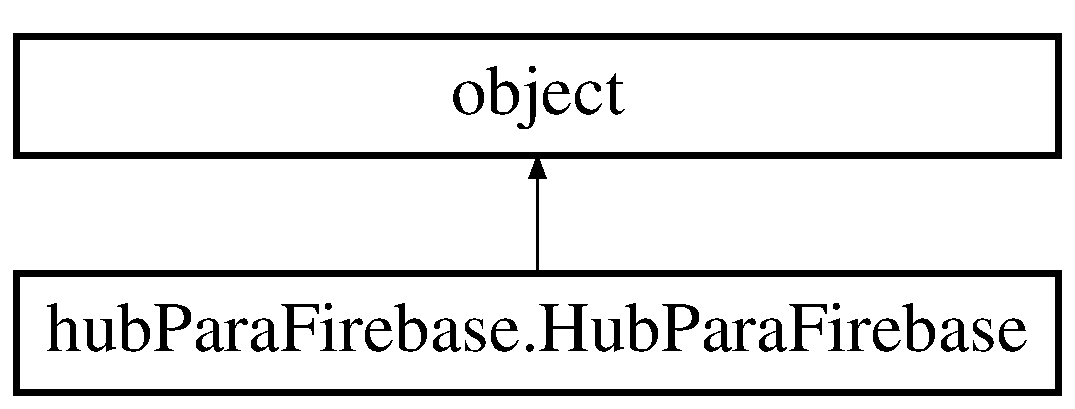
\includegraphics[height=2.000000cm]{classhub_para_firebase_1_1_hub_para_firebase}
\end{center}
\end{figure}
\subsection*{Membros públicos}
\begin{DoxyCompactItemize}
\item 
def \hyperlink{classhub_para_firebase_1_1_hub_para_firebase_a8553e4a8f4a5564e69a1ebac33e255b3}{\+\_\+\+\_\+init\+\_\+\+\_\+} (self, hub\+ID)
\begin{DoxyCompactList}\small\item\em Constructs the object. \end{DoxyCompactList}\item 
def \hyperlink{classhub_para_firebase_1_1_hub_para_firebase_a8867ea8f38db645837f1c0ab0a4b207e}{desconectar\+Firebase} (self)
\begin{DoxyCompactList}\small\item\em \{ function\+\_\+description \} \end{DoxyCompactList}\item 
def \hyperlink{classhub_para_firebase_1_1_hub_para_firebase_aec0b9ed7691e78978716075fe999019a}{mensagem\+Alarme} (self, modulo\+ID, mensagem)
\begin{DoxyCompactList}\small\item\em \{ function\+\_\+description \} \end{DoxyCompactList}\item 
def \hyperlink{classhub_para_firebase_1_1_hub_para_firebase_a269bab1a9f98ad3ef1ac4a0f31a59a57}{mensagem\+Modulo\+ON} (self, modulo\+ID)
\begin{DoxyCompactList}\small\item\em \{ function\+\_\+description \} \end{DoxyCompactList}\item 
def \hyperlink{classhub_para_firebase_1_1_hub_para_firebase_aab4023d0316ce43f1ed743aa6d02064e}{receber\+Firebase} (self, mensagem)
\begin{DoxyCompactList}\small\item\em \{ function\+\_\+description \} \end{DoxyCompactList}\item 
def \hyperlink{classhub_para_firebase_1_1_hub_para_firebase_a8c00d07d181c47e4567b602947466abe}{get\+Ultima\+Mensagem} (self)
\begin{DoxyCompactList}\small\item\em Gets the ultima mensagem. \end{DoxyCompactList}\item 
def \hyperlink{classhub_para_firebase_1_1_hub_para_firebase_a434ba152fb00900dddfaf2f61e5d78b6}{apagar\+Mensagens\+Hub} (self)
\begin{DoxyCompactList}\small\item\em \{ function\+\_\+description \} \end{DoxyCompactList}\end{DoxyCompactItemize}
\subsection*{Atributos Públicos}
\begin{DoxyCompactItemize}
\item 
{\bfseries hub\+ID}\hypertarget{classhub_para_firebase_1_1_hub_para_firebase_a13968444b5703f3c8f30c7bf14de21a8}{}\label{classhub_para_firebase_1_1_hub_para_firebase_a13968444b5703f3c8f30c7bf14de21a8}

\item 
{\bfseries app\+ID}\hypertarget{classhub_para_firebase_1_1_hub_para_firebase_a6c765d09ff060cf4a06e5f4465937b52}{}\label{classhub_para_firebase_1_1_hub_para_firebase_a6c765d09ff060cf4a06e5f4465937b52}

\item 
{\bfseries stream}\hypertarget{classhub_para_firebase_1_1_hub_para_firebase_afc660542885ce7717ef17d4ddb4f9b76}{}\label{classhub_para_firebase_1_1_hub_para_firebase_afc660542885ce7717ef17d4ddb4f9b76}

\end{DoxyCompactItemize}
\subsection*{Atributos Públicos Estáticos}
\begin{DoxyCompactItemize}
\item 
string {\bfseries hub\+ID} = \char`\"{}\char`\"{}\hypertarget{classhub_para_firebase_1_1_hub_para_firebase_a877a7af6deac7745ca493313cc812936}{}\label{classhub_para_firebase_1_1_hub_para_firebase_a877a7af6deac7745ca493313cc812936}

\item 
string {\bfseries app\+ID} = \char`\"{}\char`\"{}\hypertarget{classhub_para_firebase_1_1_hub_para_firebase_a1151963c2e4dea5ea944b2082a629a07}{}\label{classhub_para_firebase_1_1_hub_para_firebase_a1151963c2e4dea5ea944b2082a629a07}

\item 
{\bfseries firebase} = None\hypertarget{classhub_para_firebase_1_1_hub_para_firebase_aaa1bce183719a2446b9b697db2ccb45a}{}\label{classhub_para_firebase_1_1_hub_para_firebase_aaa1bce183719a2446b9b697db2ccb45a}

\item 
{\bfseries database} = None\hypertarget{classhub_para_firebase_1_1_hub_para_firebase_ad897e9d2142426f09b8154ae0e0ab374}{}\label{classhub_para_firebase_1_1_hub_para_firebase_ad897e9d2142426f09b8154ae0e0ab374}

\item 
{\bfseries gerenciador\+Mensagens\+Recebidas} = None\hypertarget{classhub_para_firebase_1_1_hub_para_firebase_ae5cbb5c32dda53f7f6a6c1b5685d2815}{}\label{classhub_para_firebase_1_1_hub_para_firebase_ae5cbb5c32dda53f7f6a6c1b5685d2815}

\item 
{\bfseries mensagens\+Recebidas} = None\hypertarget{classhub_para_firebase_1_1_hub_para_firebase_aed56c55b4e098c7c77ffee2759801901}{}\label{classhub_para_firebase_1_1_hub_para_firebase_aed56c55b4e098c7c77ffee2759801901}

\end{DoxyCompactItemize}


\subsection{Descrição detalhada}
Esta classe é responsável pela comunicação entre o H\+UB e o banco de dados firebase. 

Este módulo provem funções básicas de comunição, entretando não é responsável pela lógica usada de acordo com as mensagens.


\begin{DoxyParams}{Parâmetros}
{\em hub\+ID} & O id do hub cadastrado no banco de dados firebase \\
\hline
{\em app\+ID} & O id do app/do usuário do app no banco de dados firebase que possui o hub. \\
\hline
{\em firebase} & Objeto da classe pyrebase, responsável pela conexão com o servidor \\
\hline
{\em database} & Objeto da classe pyrebase, responsável por recuperar dados do banco de dados firebase. \\
\hline
{\em mensagens\+Recebidas} & As mensagens recebidas pelo módulo, guardadas como uma lista ordenada. \\
\hline
\end{DoxyParams}


\subsection{Documentação dos Construtores \& Destrutor}
\index{hub\+Para\+Firebase\+::\+Hub\+Para\+Firebase@{hub\+Para\+Firebase\+::\+Hub\+Para\+Firebase}!\+\_\+\+\_\+init\+\_\+\+\_\+@{\+\_\+\+\_\+init\+\_\+\+\_\+}}
\index{\+\_\+\+\_\+init\+\_\+\+\_\+@{\+\_\+\+\_\+init\+\_\+\+\_\+}!hub\+Para\+Firebase\+::\+Hub\+Para\+Firebase@{hub\+Para\+Firebase\+::\+Hub\+Para\+Firebase}}
\subsubsection[{\texorpdfstring{\+\_\+\+\_\+init\+\_\+\+\_\+(self, hub\+I\+D)}{__init__(self, hubID)}}]{\setlength{\rightskip}{0pt plus 5cm}def hub\+Para\+Firebase.\+Hub\+Para\+Firebase.\+\_\+\+\_\+init\+\_\+\+\_\+ (
\begin{DoxyParamCaption}
\item[{}]{self, }
\item[{}]{hub\+ID}
\end{DoxyParamCaption}
)}\hypertarget{classhub_para_firebase_1_1_hub_para_firebase_a8553e4a8f4a5564e69a1ebac33e255b3}{}\label{classhub_para_firebase_1_1_hub_para_firebase_a8553e4a8f4a5564e69a1ebac33e255b3}


Constructs the object. 


\begin{DoxyParams}{Parâmetros}
{\em self} & O objeto \\
\hline
{\em hub\+ID} & The hub id \\
\hline
\end{DoxyParams}


\subsection{Documentação dos métodos}
\index{hub\+Para\+Firebase\+::\+Hub\+Para\+Firebase@{hub\+Para\+Firebase\+::\+Hub\+Para\+Firebase}!apagar\+Mensagens\+Hub@{apagar\+Mensagens\+Hub}}
\index{apagar\+Mensagens\+Hub@{apagar\+Mensagens\+Hub}!hub\+Para\+Firebase\+::\+Hub\+Para\+Firebase@{hub\+Para\+Firebase\+::\+Hub\+Para\+Firebase}}
\subsubsection[{\texorpdfstring{apagar\+Mensagens\+Hub(self)}{apagarMensagensHub(self)}}]{\setlength{\rightskip}{0pt plus 5cm}def hub\+Para\+Firebase.\+Hub\+Para\+Firebase.\+apagar\+Mensagens\+Hub (
\begin{DoxyParamCaption}
\item[{}]{self}
\end{DoxyParamCaption}
)}\hypertarget{classhub_para_firebase_1_1_hub_para_firebase_a434ba152fb00900dddfaf2f61e5d78b6}{}\label{classhub_para_firebase_1_1_hub_para_firebase_a434ba152fb00900dddfaf2f61e5d78b6}


\{ function\+\_\+description \} 


\begin{DoxyParams}{Parâmetros}
{\em self} & The object\\
\hline
\end{DoxyParams}
\begin{DoxyReturn}{Retorna}
\{ description\+\_\+of\+\_\+the\+\_\+return\+\_\+value \} 
\end{DoxyReturn}
\index{hub\+Para\+Firebase\+::\+Hub\+Para\+Firebase@{hub\+Para\+Firebase\+::\+Hub\+Para\+Firebase}!desconectar\+Firebase@{desconectar\+Firebase}}
\index{desconectar\+Firebase@{desconectar\+Firebase}!hub\+Para\+Firebase\+::\+Hub\+Para\+Firebase@{hub\+Para\+Firebase\+::\+Hub\+Para\+Firebase}}
\subsubsection[{\texorpdfstring{desconectar\+Firebase(self)}{desconectarFirebase(self)}}]{\setlength{\rightskip}{0pt plus 5cm}def hub\+Para\+Firebase.\+Hub\+Para\+Firebase.\+desconectar\+Firebase (
\begin{DoxyParamCaption}
\item[{}]{self}
\end{DoxyParamCaption}
)}\hypertarget{classhub_para_firebase_1_1_hub_para_firebase_a8867ea8f38db645837f1c0ab0a4b207e}{}\label{classhub_para_firebase_1_1_hub_para_firebase_a8867ea8f38db645837f1c0ab0a4b207e}


\{ function\+\_\+description \} 


\begin{DoxyParams}{Parâmetros}
{\em self} & The object\\
\hline
\end{DoxyParams}
\begin{DoxyReturn}{Retorna}
\{ description\+\_\+of\+\_\+the\+\_\+return\+\_\+value \} 
\end{DoxyReturn}
\index{hub\+Para\+Firebase\+::\+Hub\+Para\+Firebase@{hub\+Para\+Firebase\+::\+Hub\+Para\+Firebase}!get\+Ultima\+Mensagem@{get\+Ultima\+Mensagem}}
\index{get\+Ultima\+Mensagem@{get\+Ultima\+Mensagem}!hub\+Para\+Firebase\+::\+Hub\+Para\+Firebase@{hub\+Para\+Firebase\+::\+Hub\+Para\+Firebase}}
\subsubsection[{\texorpdfstring{get\+Ultima\+Mensagem(self)}{getUltimaMensagem(self)}}]{\setlength{\rightskip}{0pt plus 5cm}def hub\+Para\+Firebase.\+Hub\+Para\+Firebase.\+get\+Ultima\+Mensagem (
\begin{DoxyParamCaption}
\item[{}]{self}
\end{DoxyParamCaption}
)}\hypertarget{classhub_para_firebase_1_1_hub_para_firebase_a8c00d07d181c47e4567b602947466abe}{}\label{classhub_para_firebase_1_1_hub_para_firebase_a8c00d07d181c47e4567b602947466abe}


Gets the ultima mensagem. 


\begin{DoxyParams}{Parâmetros}
{\em self} & The object\\
\hline
\end{DoxyParams}
\begin{DoxyReturn}{Retorna}
The ultima mensagem. 
\end{DoxyReturn}
\index{hub\+Para\+Firebase\+::\+Hub\+Para\+Firebase@{hub\+Para\+Firebase\+::\+Hub\+Para\+Firebase}!mensagem\+Alarme@{mensagem\+Alarme}}
\index{mensagem\+Alarme@{mensagem\+Alarme}!hub\+Para\+Firebase\+::\+Hub\+Para\+Firebase@{hub\+Para\+Firebase\+::\+Hub\+Para\+Firebase}}
\subsubsection[{\texorpdfstring{mensagem\+Alarme(self, modulo\+I\+D, mensagem)}{mensagemAlarme(self, moduloID, mensagem)}}]{\setlength{\rightskip}{0pt plus 5cm}def hub\+Para\+Firebase.\+Hub\+Para\+Firebase.\+mensagem\+Alarme (
\begin{DoxyParamCaption}
\item[{}]{self, }
\item[{}]{modulo\+ID, }
\item[{}]{mensagem}
\end{DoxyParamCaption}
)}\hypertarget{classhub_para_firebase_1_1_hub_para_firebase_aec0b9ed7691e78978716075fe999019a}{}\label{classhub_para_firebase_1_1_hub_para_firebase_aec0b9ed7691e78978716075fe999019a}


\{ function\+\_\+description \} 


\begin{DoxyParams}{Parâmetros}
{\em self} & The object \\
\hline
{\em modulo\+ID} & The modulo id \\
\hline
{\em mensagem} & The mensagem\\
\hline
\end{DoxyParams}
\begin{DoxyReturn}{Retorna}
\{ description\+\_\+of\+\_\+the\+\_\+return\+\_\+value \} 
\end{DoxyReturn}
\index{hub\+Para\+Firebase\+::\+Hub\+Para\+Firebase@{hub\+Para\+Firebase\+::\+Hub\+Para\+Firebase}!mensagem\+Modulo\+ON@{mensagem\+Modulo\+ON}}
\index{mensagem\+Modulo\+ON@{mensagem\+Modulo\+ON}!hub\+Para\+Firebase\+::\+Hub\+Para\+Firebase@{hub\+Para\+Firebase\+::\+Hub\+Para\+Firebase}}
\subsubsection[{\texorpdfstring{mensagem\+Modulo\+O\+N(self, modulo\+I\+D)}{mensagemModuloON(self, moduloID)}}]{\setlength{\rightskip}{0pt plus 5cm}def hub\+Para\+Firebase.\+Hub\+Para\+Firebase.\+mensagem\+Modulo\+ON (
\begin{DoxyParamCaption}
\item[{}]{self, }
\item[{}]{modulo\+ID}
\end{DoxyParamCaption}
)}\hypertarget{classhub_para_firebase_1_1_hub_para_firebase_a269bab1a9f98ad3ef1ac4a0f31a59a57}{}\label{classhub_para_firebase_1_1_hub_para_firebase_a269bab1a9f98ad3ef1ac4a0f31a59a57}


\{ function\+\_\+description \} 


\begin{DoxyParams}{Parâmetros}
{\em self} & The object \\
\hline
{\em modulo\+ID} & The modulo id\\
\hline
\end{DoxyParams}
\begin{DoxyReturn}{Retorna}
\{ description\+\_\+of\+\_\+the\+\_\+return\+\_\+value \} 
\end{DoxyReturn}
\index{hub\+Para\+Firebase\+::\+Hub\+Para\+Firebase@{hub\+Para\+Firebase\+::\+Hub\+Para\+Firebase}!receber\+Firebase@{receber\+Firebase}}
\index{receber\+Firebase@{receber\+Firebase}!hub\+Para\+Firebase\+::\+Hub\+Para\+Firebase@{hub\+Para\+Firebase\+::\+Hub\+Para\+Firebase}}
\subsubsection[{\texorpdfstring{receber\+Firebase(self, mensagem)}{receberFirebase(self, mensagem)}}]{\setlength{\rightskip}{0pt plus 5cm}def hub\+Para\+Firebase.\+Hub\+Para\+Firebase.\+receber\+Firebase (
\begin{DoxyParamCaption}
\item[{}]{self, }
\item[{}]{mensagem}
\end{DoxyParamCaption}
)}\hypertarget{classhub_para_firebase_1_1_hub_para_firebase_aab4023d0316ce43f1ed743aa6d02064e}{}\label{classhub_para_firebase_1_1_hub_para_firebase_aab4023d0316ce43f1ed743aa6d02064e}


\{ function\+\_\+description \} 


\begin{DoxyParams}{Parâmetros}
{\em self} & The object \\
\hline
{\em mensagem} & The mensagem\\
\hline
\end{DoxyParams}
\begin{DoxyReturn}{Retorna}
\{ description\+\_\+of\+\_\+the\+\_\+return\+\_\+value \} 
\end{DoxyReturn}


A documentação para esta classe foi gerada a partir do seguinte ficheiro\+:\begin{DoxyCompactItemize}
\item 
hub\+Para\+Firebase.\+py\end{DoxyCompactItemize}

\hypertarget{classhub_para_modulo_1_1_hub_para_modulo}{}\section{Referência à classe hub\+Para\+Modulo.\+Hub\+Para\+Modulo}
\label{classhub_para_modulo_1_1_hub_para_modulo}\index{hub\+Para\+Modulo.\+Hub\+Para\+Modulo@{hub\+Para\+Modulo.\+Hub\+Para\+Modulo}}


Classe para Hub\+Para\+Módulo.  


Diagrama de heranças da classe hub\+Para\+Modulo.\+Hub\+Para\+Modulo\begin{figure}[H]
\begin{center}
\leavevmode
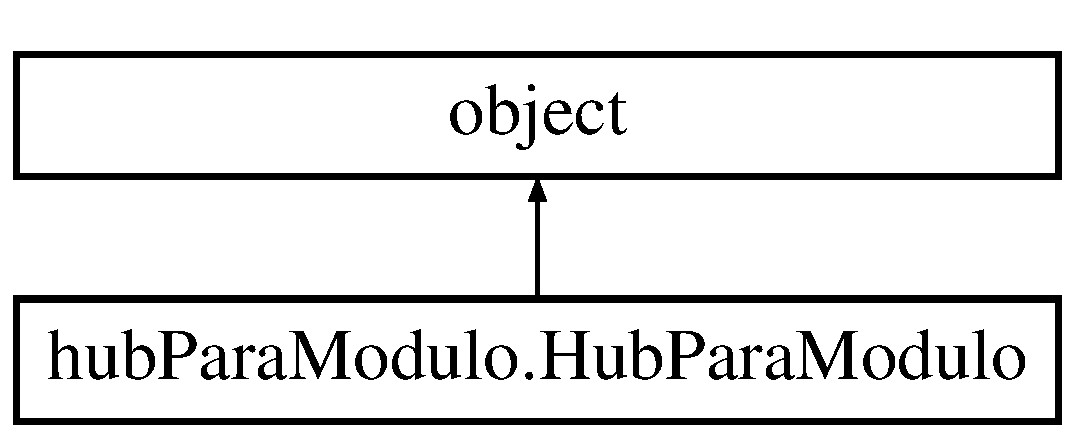
\includegraphics[height=2.000000cm]{classhub_para_modulo_1_1_hub_para_modulo}
\end{center}
\end{figure}
\subsection*{Membros públicos}
\begin{DoxyCompactItemize}
\item 
def \hyperlink{classhub_para_modulo_1_1_hub_para_modulo_abf63ddad3857ffe2c53bfa707a149c75}{\+\_\+\+\_\+init\+\_\+\+\_\+} (self, arg)
\begin{DoxyCompactList}\small\item\em Constrói o objeto. \end{DoxyCompactList}\end{DoxyCompactItemize}
\subsection*{Atributos Públicos}
\begin{DoxyCompactItemize}
\item 
{\bfseries arg}\hypertarget{classhub_para_modulo_1_1_hub_para_modulo_a0f8bf47693698c4d06489efcdfb73de9}{}\label{classhub_para_modulo_1_1_hub_para_modulo_a0f8bf47693698c4d06489efcdfb73de9}

\end{DoxyCompactItemize}


\subsection{Descrição detalhada}
Classe para Hub\+Para\+Módulo. 

\subsection{Documentação dos Construtores \& Destrutor}
\index{hub\+Para\+Modulo\+::\+Hub\+Para\+Modulo@{hub\+Para\+Modulo\+::\+Hub\+Para\+Modulo}!\+\_\+\+\_\+init\+\_\+\+\_\+@{\+\_\+\+\_\+init\+\_\+\+\_\+}}
\index{\+\_\+\+\_\+init\+\_\+\+\_\+@{\+\_\+\+\_\+init\+\_\+\+\_\+}!hub\+Para\+Modulo\+::\+Hub\+Para\+Modulo@{hub\+Para\+Modulo\+::\+Hub\+Para\+Modulo}}
\subsubsection[{\texorpdfstring{\+\_\+\+\_\+init\+\_\+\+\_\+(self, arg)}{__init__(self, arg)}}]{\setlength{\rightskip}{0pt plus 5cm}def hub\+Para\+Modulo.\+Hub\+Para\+Modulo.\+\_\+\+\_\+init\+\_\+\+\_\+ (
\begin{DoxyParamCaption}
\item[{}]{self, }
\item[{}]{arg}
\end{DoxyParamCaption}
)}\hypertarget{classhub_para_modulo_1_1_hub_para_modulo_abf63ddad3857ffe2c53bfa707a149c75}{}\label{classhub_para_modulo_1_1_hub_para_modulo_abf63ddad3857ffe2c53bfa707a149c75}


Constrói o objeto. 


\begin{DoxyParams}{Parâmetros}
{\em self} & O objeto \\
\hline
{\em arg} & O argumento \\
\hline
\end{DoxyParams}


A documentação para esta classe foi gerada a partir do seguinte ficheiro\+:\begin{DoxyCompactItemize}
\item 
hub\+Para\+Modulo.\+py\end{DoxyCompactItemize}

\hypertarget{classled_manager_1_1_led_manager}{}\section{Referência à classe led\+Manager.\+Led\+Manager}
\label{classled_manager_1_1_led_manager}\index{led\+Manager.\+Led\+Manager@{led\+Manager.\+Led\+Manager}}


Classe para o \hyperlink{classled_manager_1_1_led_manager}{Led\+Manager}.  


Diagrama de heranças da classe led\+Manager.\+Led\+Manager\begin{figure}[H]
\begin{center}
\leavevmode
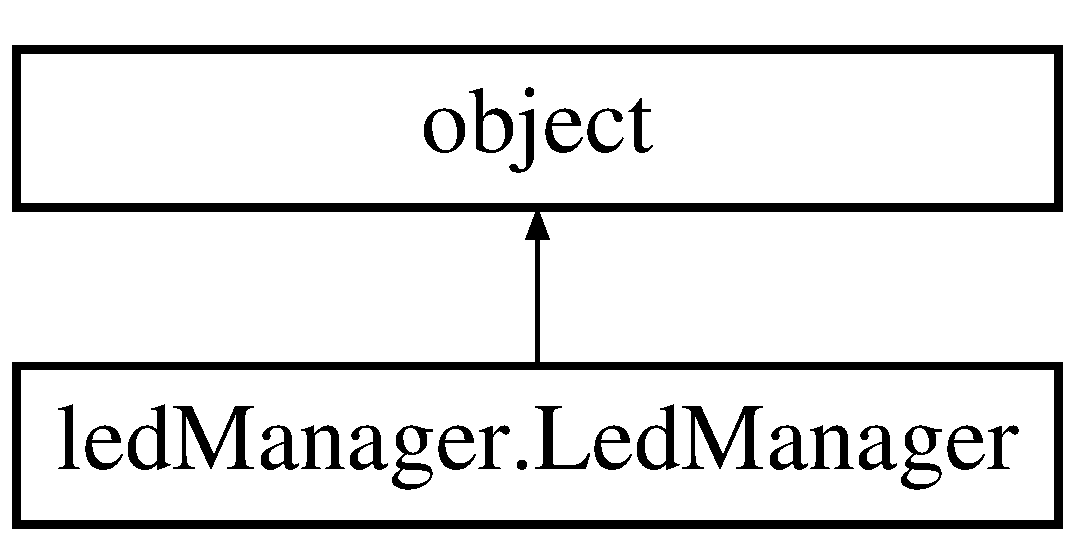
\includegraphics[height=2.000000cm]{classled_manager_1_1_led_manager}
\end{center}
\end{figure}
\subsection*{Membros públicos}
\begin{DoxyCompactItemize}
\item 
def \hyperlink{classled_manager_1_1_led_manager_a5bc4f172c79144377da875a1290a7dbd}{\+\_\+\+\_\+init\+\_\+\+\_\+} (self)
\begin{DoxyCompactList}\small\item\em Método de inicialização para o \hyperlink{classled_manager_1_1_led_manager}{Led\+Manager}. \end{DoxyCompactList}\item 
def \hyperlink{classled_manager_1_1_led_manager_ace03fe1a941d4b5f4d7e9d3c47964e36}{procura\+Significado} (status)
\begin{DoxyCompactList}\small\item\em Dado um {\ttfamily status}, método retorna uma cor. \end{DoxyCompactList}\item 
def \hyperlink{classled_manager_1_1_led_manager_aa6376276d32605b1958f941a05ed0a3d}{ligar\+Led} (rgb)
\begin{DoxyCompactList}\small\item\em Método usa biblioteca de manipulação de hardware da raspberry para acionar led. \end{DoxyCompactList}\item 
def \hyperlink{classled_manager_1_1_led_manager_a14e59e953d64be5fe1e58e7ecbfdbe7c}{desligar\+Led} ()
\begin{DoxyCompactList}\small\item\em Desliga o led. \end{DoxyCompactList}\end{DoxyCompactItemize}
\subsection*{Atributos Públicos Estáticos}
\begin{DoxyCompactItemize}
\item 
dictionary {\bfseries cores} = \{\}\hypertarget{classled_manager_1_1_led_manager_a1ca6df605b67f9dac8a8775fd10c540e}{}\label{classled_manager_1_1_led_manager_a1ca6df605b67f9dac8a8775fd10c540e}

\end{DoxyCompactItemize}


\subsection{Descrição detalhada}
Classe para o \hyperlink{classled_manager_1_1_led_manager}{Led\+Manager}. 

O \hyperlink{classled_manager_1_1_led_manager}{Led\+Manager} tem seus métodos chamados pelo método acionar\+Led do H\+UB. Esta classe deve servir de apoio para a classe correspondente no H\+UB. Não há um loop principal.


\begin{DoxyParams}{Parâmetros}
{\em cores} & Dicionário que contém os status e cores, onde para cada status há uma cor correspondente \\
\hline
\end{DoxyParams}
\begin{DoxyWarning}{Aviso}
Adicionar os atributos dessa classe correspondentes a classes necessárias para de fato acionar o led em hardware, e inicializar os mesmos em init. 
\end{DoxyWarning}


\subsection{Documentação dos Construtores \& Destrutor}
\index{led\+Manager\+::\+Led\+Manager@{led\+Manager\+::\+Led\+Manager}!\+\_\+\+\_\+init\+\_\+\+\_\+@{\+\_\+\+\_\+init\+\_\+\+\_\+}}
\index{\+\_\+\+\_\+init\+\_\+\+\_\+@{\+\_\+\+\_\+init\+\_\+\+\_\+}!led\+Manager\+::\+Led\+Manager@{led\+Manager\+::\+Led\+Manager}}
\subsubsection[{\texorpdfstring{\+\_\+\+\_\+init\+\_\+\+\_\+(self)}{__init__(self)}}]{\setlength{\rightskip}{0pt plus 5cm}def led\+Manager.\+Led\+Manager.\+\_\+\+\_\+init\+\_\+\+\_\+ (
\begin{DoxyParamCaption}
\item[{}]{self}
\end{DoxyParamCaption}
)}\hypertarget{classled_manager_1_1_led_manager_a5bc4f172c79144377da875a1290a7dbd}{}\label{classled_manager_1_1_led_manager_a5bc4f172c79144377da875a1290a7dbd}


Método de inicialização para o \hyperlink{classled_manager_1_1_led_manager}{Led\+Manager}. 

O atributo cores deve ser inicializado aqui, de modo que cada status tenha uma cor correspondente. Levando em conta que {\ttfamily cores} é um dicionário.

\begin{DoxyWarning}{Aviso}
Inicializar instâncias de classes necessárias depois aqui. 

Possível melhoria\+: pegar cores de arquivo de configuração. 
\end{DoxyWarning}


\subsection{Documentação dos métodos}
\index{led\+Manager\+::\+Led\+Manager@{led\+Manager\+::\+Led\+Manager}!desligar\+Led@{desligar\+Led}}
\index{desligar\+Led@{desligar\+Led}!led\+Manager\+::\+Led\+Manager@{led\+Manager\+::\+Led\+Manager}}
\subsubsection[{\texorpdfstring{desligar\+Led()}{desligarLed()}}]{\setlength{\rightskip}{0pt plus 5cm}def led\+Manager.\+Led\+Manager.\+desligar\+Led (
\begin{DoxyParamCaption}
{}
\end{DoxyParamCaption}
)}\hypertarget{classled_manager_1_1_led_manager_a14e59e953d64be5fe1e58e7ecbfdbe7c}{}\label{classled_manager_1_1_led_manager_a14e59e953d64be5fe1e58e7ecbfdbe7c}


Desliga o led. 

Simples assim.

O método deve usar uma biblioteca para manipulação de hardware da raspberry e enviar para o led um comando que apropriadamente o desliga.

\begin{DoxyReturn}{Retorna}
O valor de retorno sempre será {\ttfamily N\+U\+LL}. 
\end{DoxyReturn}
\index{led\+Manager\+::\+Led\+Manager@{led\+Manager\+::\+Led\+Manager}!ligar\+Led@{ligar\+Led}}
\index{ligar\+Led@{ligar\+Led}!led\+Manager\+::\+Led\+Manager@{led\+Manager\+::\+Led\+Manager}}
\subsubsection[{\texorpdfstring{ligar\+Led(rgb)}{ligarLed(rgb)}}]{\setlength{\rightskip}{0pt plus 5cm}def led\+Manager.\+Led\+Manager.\+ligar\+Led (
\begin{DoxyParamCaption}
\item[{}]{rgb}
\end{DoxyParamCaption}
)}\hypertarget{classled_manager_1_1_led_manager_aa6376276d32605b1958f941a05ed0a3d}{}\label{classled_manager_1_1_led_manager_aa6376276d32605b1958f941a05ed0a3d}


Método usa biblioteca de manipulação de hardware da raspberry para acionar led. 

O método deve usar uma biblioteca para manipulação de hardware da raspberry e enviar para o led um comando que apropriadamente o coloque na cor indicada.


\begin{DoxyParams}{Parâmetros}
{\em rgb} & O valor de rbg para o led. É uma intância da classe \hyperlink{classled_manager_1_1_r_g_b}{R\+GB}.\\
\hline
\end{DoxyParams}
\begin{DoxyReturn}{Retorna}
O valor de retorno sempre será {\ttfamily N\+U\+LL}. 
\end{DoxyReturn}
\index{led\+Manager\+::\+Led\+Manager@{led\+Manager\+::\+Led\+Manager}!procura\+Significado@{procura\+Significado}}
\index{procura\+Significado@{procura\+Significado}!led\+Manager\+::\+Led\+Manager@{led\+Manager\+::\+Led\+Manager}}
\subsubsection[{\texorpdfstring{procura\+Significado(status)}{procuraSignificado(status)}}]{\setlength{\rightskip}{0pt plus 5cm}def led\+Manager.\+Led\+Manager.\+procura\+Significado (
\begin{DoxyParamCaption}
\item[{}]{status}
\end{DoxyParamCaption}
)}\hypertarget{classled_manager_1_1_led_manager_ace03fe1a941d4b5f4d7e9d3c47964e36}{}\label{classled_manager_1_1_led_manager_ace03fe1a941d4b5f4d7e9d3c47964e36}


Dado um {\ttfamily status}, método retorna uma cor. 

Tão simples quanto na descrição resumida. O método deve receber um status e devolver uma cor. Nada mais é do que a aplicação do dicionário desta classe.


\begin{DoxyParams}{Parâmetros}
{\em status} & O Estado que deseja-\/se saber a cor.\\
\hline
\end{DoxyParams}
\begin{DoxyReturn}{Retorna}
Retorna a cor, do tipo \hyperlink{classled_manager_1_1_r_g_b}{R\+GB}. 
\end{DoxyReturn}


A documentação para esta classe foi gerada a partir do seguinte ficheiro\+:\begin{DoxyCompactItemize}
\item 
led\+Manager.\+py\end{DoxyCompactItemize}

\hypertarget{classled_manager_1_1_r_g_b}{}\section{Referência à classe led\+Manager.\+R\+GB}
\label{classled_manager_1_1_r_g_b}\index{led\+Manager.\+R\+GB@{led\+Manager.\+R\+GB}}


Classe para rgb.  


Diagrama de heranças da classe led\+Manager.\+R\+GB\begin{figure}[H]
\begin{center}
\leavevmode
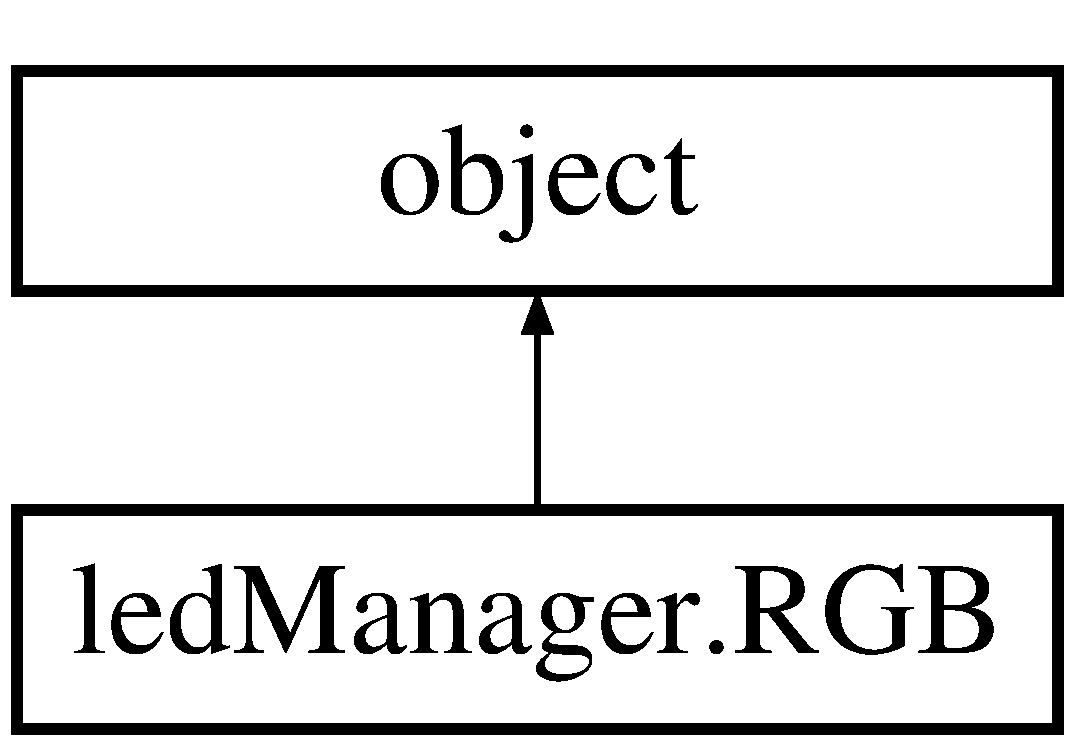
\includegraphics[height=2.000000cm]{classled_manager_1_1_r_g_b}
\end{center}
\end{figure}
\subsection*{Membros públicos}
\begin{DoxyCompactItemize}
\item 
def \hyperlink{classled_manager_1_1_r_g_b_a871e398f9266f95ffa795ae7d7700d53}{\+\_\+\+\_\+init\+\_\+\+\_\+} (self, red, green, blue)
\begin{DoxyCompactList}\small\item\em Inicializa uma cor. \end{DoxyCompactList}\end{DoxyCompactItemize}
\subsection*{Atributos Públicos}
\begin{DoxyCompactItemize}
\item 
{\bfseries red}\hypertarget{classled_manager_1_1_r_g_b_a13d2a549b0d1b8ae4544e5fe161f5ed5}{}\label{classled_manager_1_1_r_g_b_a13d2a549b0d1b8ae4544e5fe161f5ed5}

\item 
{\bfseries green}\hypertarget{classled_manager_1_1_r_g_b_afa5083980155e25e5af80aa4372bbcdc}{}\label{classled_manager_1_1_r_g_b_afa5083980155e25e5af80aa4372bbcdc}

\item 
{\bfseries blue}\hypertarget{classled_manager_1_1_r_g_b_adf44b49c16c2fdfd9aec57ba198422fc}{}\label{classled_manager_1_1_r_g_b_adf44b49c16c2fdfd9aec57ba198422fc}

\end{DoxyCompactItemize}
\subsection*{Atributos Públicos Estáticos}
\begin{DoxyCompactItemize}
\item 
int {\bfseries red} = 0\hypertarget{classled_manager_1_1_r_g_b_a37944e5625887644ac5ab4338839a3d6}{}\label{classled_manager_1_1_r_g_b_a37944e5625887644ac5ab4338839a3d6}

\item 
int {\bfseries green} = 0\hypertarget{classled_manager_1_1_r_g_b_a4473532261cc1d890e7027793ecb12ae}{}\label{classled_manager_1_1_r_g_b_a4473532261cc1d890e7027793ecb12ae}

\item 
int {\bfseries blue} = 0\hypertarget{classled_manager_1_1_r_g_b_a0236b1f9c992ff71353b03bd5f0418b7}{}\label{classled_manager_1_1_r_g_b_a0236b1f9c992ff71353b03bd5f0418b7}

\end{DoxyCompactItemize}


\subsection{Descrição detalhada}
Classe para rgb. 

Essa classe nada mais é do que o equivalente a uma struct em c. Só armazena de forma rezumida uma cor \hyperlink{classled_manager_1_1_r_g_b}{R\+GB}.


\begin{DoxyParams}{Parâmetros}
{\em red} & Cor vermelha armazenada, inteiro, com valores indo de 0 a 255 \\
\hline
{\em green} & Cor verde armazenada, inteiro, com valores indo de 0 a 255 \\
\hline
{\em blue} & Cor azul armazenada, inteiro, com valores indo de 0 a 255 \\
\hline
\end{DoxyParams}


\subsection{Documentação dos Construtores \& Destrutor}
\index{led\+Manager\+::\+R\+GB@{led\+Manager\+::\+R\+GB}!\+\_\+\+\_\+init\+\_\+\+\_\+@{\+\_\+\+\_\+init\+\_\+\+\_\+}}
\index{\+\_\+\+\_\+init\+\_\+\+\_\+@{\+\_\+\+\_\+init\+\_\+\+\_\+}!led\+Manager\+::\+R\+GB@{led\+Manager\+::\+R\+GB}}
\subsubsection[{\texorpdfstring{\+\_\+\+\_\+init\+\_\+\+\_\+(self, red, green, blue)}{__init__(self, red, green, blue)}}]{\setlength{\rightskip}{0pt plus 5cm}def led\+Manager.\+R\+G\+B.\+\_\+\+\_\+init\+\_\+\+\_\+ (
\begin{DoxyParamCaption}
\item[{}]{self, }
\item[{}]{red, }
\item[{}]{green, }
\item[{}]{blue}
\end{DoxyParamCaption}
)}\hypertarget{classled_manager_1_1_r_g_b_a871e398f9266f95ffa795ae7d7700d53}{}\label{classled_manager_1_1_r_g_b_a871e398f9266f95ffa795ae7d7700d53}


Inicializa uma cor. 

Ao chamar essa função, a cor é inicializada e utilizada nessa instância.


\begin{DoxyParams}{Parâmetros}
{\em self} & O objeto \\
\hline
{\em red} & Cor vermelha, inteiro, com valores indo de 0 a 255 \\
\hline
{\em green} & Cor verde, inteiro, com valores indo de 0 a 255 \\
\hline
{\em blue} & Cor Azul, inteiro, com valores indo de 0 a 255 \\
\hline
\end{DoxyParams}


A documentação para esta classe foi gerada a partir do seguinte ficheiro\+:\begin{DoxyCompactItemize}
\item 
led\+Manager.\+py\end{DoxyCompactItemize}

%--- End generated contents ---

% Index
\backmatter
\newpage
\phantomsection
\clearemptydoublepage
\addcontentsline{toc}{chapter}{Índice}
\printindex

\end{document}
